% !TEX program = xelatex
\documentclass[UTF8,zihao=-4,]{ctexart}
\usepackage{texproposal}


% 定义所有的图片文件在 figures 子目录下
\graphicspath{{figures/}}
\makeindex
\begin{document}
%********英文标题**********
\begin{center}
	{\zihao{-2}\bfseries\color{tsTitle}\etstitle}\\[8mm]
	{\zihao{-4}\rmfamily
	Zhennan Li\footnote{Innovation Center of Undergraduates, Chongqing University, Chongqing, China, 400000}\footnote{Contact: i@nanmu.me}\hskip1em
	Chenyu Wu\footnotemark[1]\hskip1em
	Chunlei Liu\footnotemark[1]\hskip1em
	Pinyong Zhao\footnotemark[1]\footnote{Cite this DOI:\href{https://doi.org/10.5281/zenodo.154440}{10.5281/zenodo.154440}, if in need. This work could be a proposal prototype for \LaTeX promotion in Chinese universities, source code available at \url{https://github.com/CQUtug/TeXProposal}.}
	}
\end{center}
\vspace{\stretch{1}}
\def\abstractname{Abstract}
\begin{abstract}
	\mdseries\etsabstract
\end{abstract}
\vspace{\stretch{3}}
\begin{multicols}{2}[
	\setlength{\columnseprule}{.4pt}
	\setlength{\columnsep}{18pt}]
	\listofecontents
\end{multicols}
\vspace{\stretch{1}}
\pagework % 单双面打印适配
%*******中文标题**********
\author{%
	李振楠\footnote{重庆大学2012级材料学院本科毕业生,材料创新实践班结业成员,\href{https://github.com/nanmu42/CQUThesis}{\cquthesis} 作者。}\hskip\ccwd%
	武晨宇\footnote{重庆大学2012级材料学院本科毕业生,人文与社会科学创新实践班结业成员,\href{http://jq.qq.com/?_wv=1027&k=2HvYu95}{重庆大学\TeX 用户组}秘书。}\hskip\ccwd%
	刘春蕾\footnote{重庆大学2015级数统学院本科生,人文与社会科学创新实践班成员,\href{http://jq.qq.com/?_wv=1027&k=2HvYu95}{重庆大学\TeX 用户组}秘书。}\hskip\ccwd%
	赵品勇\footnote{指导老师,重庆大学大学生创新实践中心负责人。}}%author
\title{\sffamily\heiti\color{tsTitle}\tstitle\footnote{如有需要,可使用DOI:\href{https://doi.org/10.5281/zenodo.154440}{10.5281/zenodo.154440}引用本文。本文可作为类似提议的参考,如有需求,源代码位于\url{https://github.com/CQUtug/TeXProposal}。}}
\maketitle
\vspace{\stretch{1}}
\def\abstractname{摘\hskip\ccwd 要}
\begin{abstract}
\tsabstract
\end{abstract}
\vspace{\stretch{3}}
\begin{multicols}{2}[
 \setlength{\columnseprule}{.4pt}
 \setlength{\columnsep}{18pt}]
 \tableofcontents
\end{multicols}
\vspace{\stretch{1}}
\pagework % 单双面打印适配

%=======正文部分=========
%****第一章:引子*****
\section{引言}[Introduction]

\ppt{本提案与“双一流”建设之联系}
“必人才日出,然后事业日新;必事业日新,然后生机永畅。”

我国即将实行的“双一流大学”建设计划,是事关未来教育发展的重要改革,其一主要任务——“培养拔尖创新人才。突出人才培养的核心地位,着力培养具有国家使命感和社会责任心,富有创新精神和实践能力的各类创新型、应用型、复合型的优秀人才。”

重庆大学作为国内知名学府,在建设“双一流高校”的历程中,自当紧跟教育改革浪潮,围绕改革目标,通过人才培养与管理机制的创新,努力挖掘学生的的创新潜质,调动创新意识,营造创新氛围,培养一批拥有全球视野、掌握核心竞争力的拔尖创新人才。

\ppt{塑造自由创新的学术写作环境}
从大处着眼——拔尖创新人才的培养,需要充分的资源和自由的环境。从小处着手——学术论文写作是学生学习研究的核心部分,也是创新型人才的基本素养。因此,自由创新的论文写作环境的塑造,是值得提倡的着手点。
第一,为学术论文写作提供全面、自由的支持,将解放学生更多思考及精力投入于学习和研究本身。
第二,写作是学术“日常”,若能使创新能力培养与学术写作糅合,必能有效掀动校园创新之风。
第三,由于历史原因,我国在学术写作工具及资源的多样化支持上,始终未与学术界及西方高校接轨;在国内重点高校中,我校也未能走在前列,这一点亟待我辈追赶。
言而总之,我校在自由创新的学术写作环境的塑造方面,是大有可为的。


\ppt{\TeX 与Word:学术写作}
上世纪 80 年代末 Word 出现以前,排版语言 \TeX 是高校及学术界学术论文写作的绝对主流。Word 出现以后时至今日,\TeX  与 Word 优势互补,成为学术写作界并行的两大标准。然而,由于我国信息革命起步较晚,低门槛的 Word 迅速进入高校成为单一标准,依旧在学术界通行的老传统\TeX 却仅为少数师生所知,其独特功能和魅力没能在国内得以充分体现。这在一定程度上限制了师生在学术写作领域与国际学术界的对接。

\ppt{\TeX:编程思维和创新意识}
除此之外,\TeX 对于学生编程思维和创新意识的培养亦有所增益。这是因为在\TeX 写作过程中,其类似于编程语言的问题解决方式,问题发现和处理的多样化、逻辑性和创造性,使得\TeX 用户在写作过程中有效锻炼了其编程思维、创新意识。

\ppt*{引入\TeX 助力创新型人才培养}
本提案从介绍排版系统\TeX 的背景及特点开始,从研究生期刊论文投稿以及毕业生毕业论文排版工作这两个维度阐述了引入\TeX 作为一种与MS Word平行的写作系统的优势和必要性,最终提出一套基于我校实际情况、有效可行的实施方案。


%****第二章:我们需要TeX*****
\section{我们需要\TeX}[Need for \TeX ]
\subsection{什么是\TeX ,以及它能做什么}[\TeX , and the Talent Show]\label{sec:whatistex}
\TeX ,是科研界论文排版的事实标准。

\ppt{\TeX:定义}
\TeX ,读作“泰克”,是一种计算机排版系统,大部分由高德纳教授\footnote{Donald Ervin Knuth,斯坦福大学终身荣誉教授,他在计算机方面有着极深的造诣和卓越的贡献,著有《计算机编程的艺术》\cite{Knuth:ACPV1,Knuth:ACPV2,Knuth:ACPV3},这是一部计划有7卷(目前写至第5卷)之多的鸿篇巨著,内容涉及程序算法和编译。此外,他在文字排版领域也有诸多贡献,\TeX 便是其中之一。}设计和编写。这个发布于1978年(并且不断更新)的系统在设计之初就被赋予了两个使命:
1. 让任何人都能以极低的代价完成高质量的排版工作,哪怕你正打算进行排版的是一部书籍;
2. 系统本身要有着足够的一致性,使得同一份文件能在不同的计算机上实现相同的结果。\TeX 是自由软件,任何人都可以无偿使用它,而且,如果你愿意,你可以为它的开发工作作出自己的贡献。

然而,\TeX 这个词汇的外延还没有止步于此。由于\TeX 语言本身并不是那么容易理解和领会,在\TeX 发行之初,真正能驾驭它进行排版工作的人并不多,为了解决这个问题,1985年,Leslie Lamport\footnote{美国计算机学家,1941年生,2013年获得图灵奖。在2000年前后加入了微软研究院,此后,微软的MS Office Word在数学公式排版方面有了明显的提升。}将\TeX 的语言进行组织和包装,开发出了更容易理解和使用的\LaTeX ,从那时起,越来越多的人(尤其是科研工作者和相关出版社)开始使用\LaTeX 作为排版的工具\footnote{值得注意的是,Microsoft Word的第一个版本在1983年发行,当时,局限于有限的排版能力(特别是数学方程的排版)以及其商业软件的角色,大部分科研人员仍然选择了\LaTeX 。}。

\ppt{\TeX:衍生}
随着人们需求的变革和计算机水平的发展,除了\LaTeX 以外,\TeX 有了更多的衍生:

\begin{itemize}
	\item 为了让排版后的文件直接输出为PDF格式,人们开发了pdf\LaTeX ;
	\item \TeX  在设计之初并没有考虑支持全球语言(例如中日韩文),\XeLaTeX 应运而生;
	\item 结合了lua语言的\LuaLaTeX 更加智能,能够完成要求极其苛刻的排版任务。
\end{itemize}

\ppt{\TeX 与Word:特征与比较}
作为功能有所重叠的工具,\TeX 和MS Word不免被人们相互比较。很多年以来,这个问题在国内外的各个\TeX 或Office社区(\href{www.ctex.org}{C\TeX 社区}、\href{tex.stackexchange.com}{\TeX on Stackexchange})和综合性问答平台(\href{www.quora.com}{Quora}、\href{www.zhihu.com}{知乎})上都有提及\footnote{点击名称可直接访问,本条特性适用于本文档的PDF版本。},已然成为老生常谈。

务实地讲,工具是否强大,与工具本身性质和用户对工具的熟悉程度息息相关。在这里,我们先假设用户对\TeX 和Word都很熟悉,即具备一定实际工作能力,在此条件下,我们对\TeX 和MS Word本身性质进行比较,如\autoref{fig:tex-word-diff}所示。

\begin{figure}[tbh]
\centering
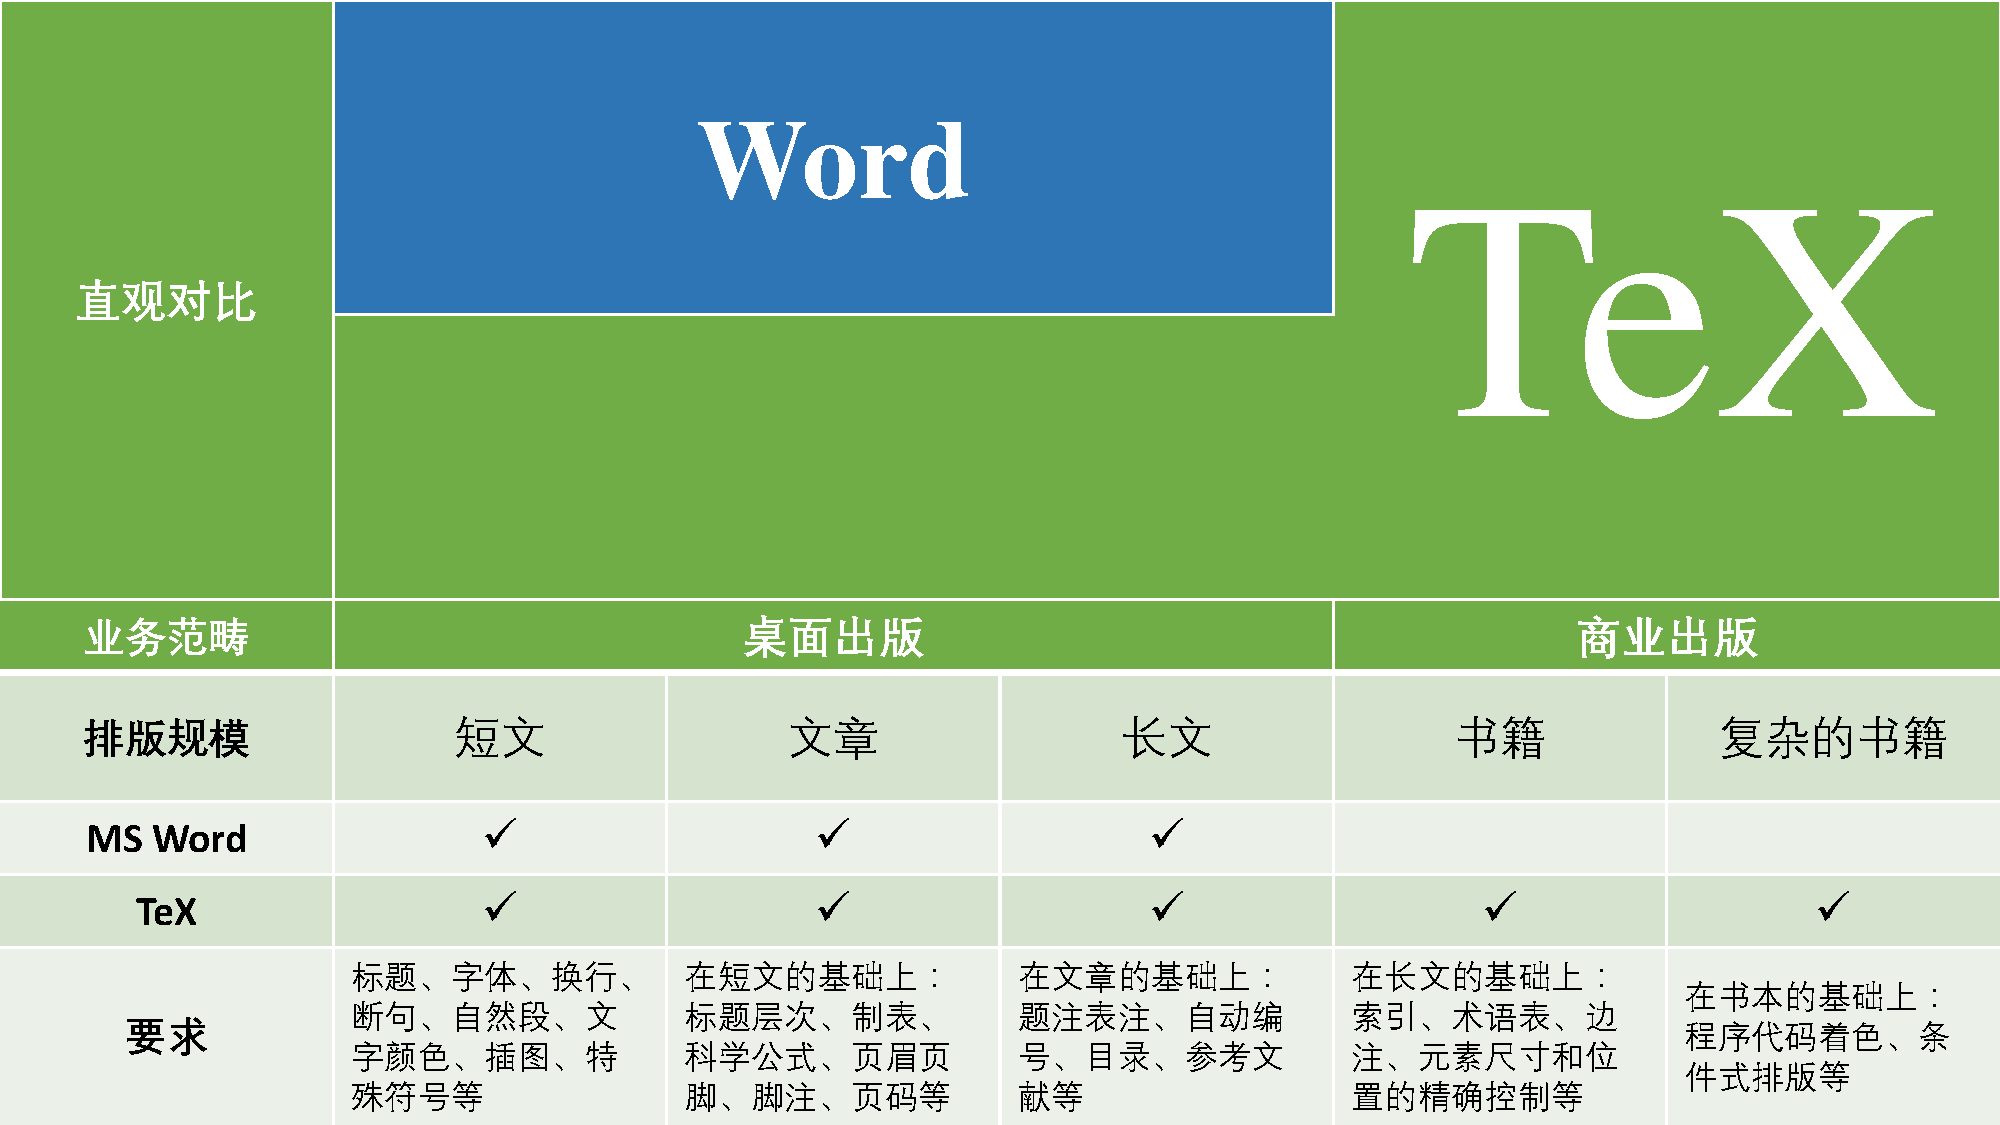
\includegraphics[width=\linewidth]{TeX-Word-Diff}
\caption{\TeX 和MS Word在设计意图上的比较}
\label{fig:tex-word-diff}
\end{figure}

通过比较,我们能得出以下初步结论:
1. \TeX 作为一套商业出版\footnote{\TeX 并不是商业软件,这里是指其设计意图面向商业出版。}软件,能够完成从短文到复杂书籍几乎所有排版规模的排版工作;
2. MS Word作为一套桌面出版软件,以满足大部分个人用户和公司的需求为设计目的,能够完成规模从短文到长文的排版工作。
但是,我们需要注意到,得益于MS Word的“所见即所得”(What you see is what you get.)的机制\footnote{\TeX 的机制为“所想即所得”,即What you think is what you get.},在对短文和文章(大部分用户的使用情况)进行排版时会比\TeX 有着更高的效率,再考虑到微软大力的市场推广行为以及软件学习成本\footnote{不熟悉英文的用户是很难学习\TeX 的。Word是汉化过的图形界面软件,对于不熟悉英文、一般只进行短文和文章规模的编辑和排版的用户来说,是一个非常自然的选择。},MS Word风靡于世便是意料之中的事情了。

\ppt{\TeX 与Word:学术写作}
然而,学术写作,是一个长文级别的排版工作。

无论是毕业论文,还是期刊投稿,学校或出版社都对论文有着很高的排版要求,这些要求往往十分细致,例如字号、字体、间距、各级标题格式、页眉页脚、目录成分、附录要求、参考文献引用标准和标示符号等等。\TeX 可以很容易地满足这类细致和繁多的排版要求,并且,通过将“如何满足这些要求”的方法包装为\TeX 模板文件,用户可以通过直接引用模板文件的方式来完成排版,免去了自己配置和调校格式的烦恼。

\ppt{\cquthesis:介绍}
让我们以我校李振楠同学开发的\cquthesis 为例,\href{https://github.com/nanmu42/CQUThesis}{\cquthesis} 是一个缩略语,表示的是\href{https://github.com/nanmu42/CQUThesis}{\textbf{C}hong\textbf{Q}ing \textbf{U}niversity \textbf{Thesis}},是重庆大学毕业论文的\TeX 模板,支持学士、硕士、博士论文的排版。合理使用该宏包可以大大减轻重庆大学毕业生在毕业论文撰写过程中的排版工作量。CQUThesis根据重庆大学《重庆大学本科设计(论文)撰写规范化要求(2007年修订版)》和《重庆大学博士、硕士论文撰写格式标准(2007年修订版)》编写,力求合规,简洁,易于实现,用户友好。模板的宣传海报如\autoref{fig:cquthesis-poster}所示。

\begin{figure}[tbh]
\centering

\includegraphics[angle=270,width=\linewidth,]{figures/CQUThesis-poster}
\caption[\cquthesis 宣传海报]{\cquthesis 宣传海报,本文档电子版可无限放大以查看细节}
\label{fig:cquthesis-poster}
\end{figure}

\ppt{\cquthesis:特色}
\cquthesis 具有如下特色:
\begin{itemize}
	\item 支持重庆大学本科(文学、理工)、硕士(学术、专业)、博士的毕业论文格式;
	\item 内置封面、目录、索引、授权书等论文部件,可按需自动生成;
	\item 自动侦测文档页数,生成相应的单面打印/双面打印PDF文件;
	\item 预置一批优化过的宏包和小功能,包含中英双语题注及配套图录、表录,国际标准单位、化学式支持、三线表等,可按需开启;
	\item 支持基于cwl文件的代码着色和补全,\texttt{makefile}功能能够在Linux, Mac, Windows三平台通用,可以轻松实现一键快速编译。
\end{itemize}

\ppt{\cquthesis:示例及优势}
举个例子,在\cquthesis 中,用户在排版封面和摘要时,只需要以“填空”的形式给出信息,余下的所有工作都由\TeX 和 \cquthesis 来完成,示例代码如下(只需填空,代码已预置):

\lstinputlisting[style=lstStyleLaTeX]{scripts/cover.tex}

即可得到如\autoref{fig:CQU-Example}所示的中英论文封面以及摘要。

\begin{figure}[p]
	\centering
	\begin{tabular}{|c@{}|c@{}|}
		\hline
		
\includegraphics[page=1,width=.5\textwidth]{CQU-Example} & 
		
\includegraphics[page=2,width=.5\textwidth]{CQU-Example} \\
		\hline
		
\includegraphics[page=3,width=.5\textwidth]{CQU-Example} & 
		
\includegraphics[page=4,width=.5\textwidth]{CQU-Example} \\
		\hline
	\end{tabular}
	\caption[\cquthesis 中英论文封面以及摘要示例]{\cquthesis 中英论文封面以及摘要示例,本文档电子版可无限放大以查看细节,良好的矢量图形支持是\TeX 的一个特性。 }
	\label{fig:CQU-Example}
\end{figure}

\ppt{\cquthesis:示例及优势}
另外一个例子是,根据重庆大学《重庆大学本科设计(论文)撰写规范化要求(2007年修订版)》和《重庆大学博士、硕士论文撰写格式标准(2007年修订版)》的规定,本科生的论文在达到70页(研究生的标准为60页)后,需要改为采用双面打印。这时,页面的页眉页脚内容以及装订线位置都需要进行调整\footnote{需要调整的还有章节右开(而且还是可选项)、正文右开等等。},\cquthesis 会在排版时预测论文页数,自动确定打印方式是双面还是单面,进而对页眉页脚等各个项目进行自动调整。这一切在Word中需要手动进行\footnote{MS Word同样具有可编程特性,即VBA,这个问题对于Word高手来说确实一样可以完成自动化,但是VBA的分发以及使用并没有\TeX 模板这么便利,何况,自动判定单双面打印只是\cquthesis 的功能的一小部分。}。

\ppt{\TeX:深度定义}
在这一节的末尾,让我们总结一下,迄今为止,我们对\TeX 的认识:
\begin{itemize}
	\item \TeX 是一个任何人都可以无偿使用的,面向商业出版的自由软件;
	\item \TeX 和MS Word并不存在高下之分,它们的设计理念和目标邻域不同;
	\item \TeX 在长文排版上较Word有优势,但在短文方面有劣势;
	\item Word面向桌面出版而设计,不难满足对书籍和复杂文档的排版需求;
	\item 得益于可编程的特性,\TeX 能够满足许多复杂的,基于条件的排版要求;
	\item 在优秀模板的支持下,即使是\TeX 初学者也能按部就班地完成格式规范,索引齐全,美观大方的排版工作。
\end{itemize}
\subsection{期刊投稿对\TeX 的需求}[\TeX in Academic Writing]\label{sec:jounaldemands}

\ppt{\TeX 与Word:地位变迁}
自1977年诞生以来,\TeX 及衍生的 \LaTeX, pdf\LaTeX, \XeLaTeX 等便因其高效高质的断行能力、数学式化学式支持、参考文献支持等优良特性迅速赢得出版业与学术界的用户的心。到了20世纪90年代,微软的Office Word终于具有了一定实力,从\TeX 阵营中分流了大部分仅有桌面出版需求的用户,但在学术界,\TeX 的强大功能及传统地位仍然难以撼动。

\ppt{\TeX:学术界地位}
当今,\TeX 与 Word 并行于当代国际主流学术界,几乎所有的学术机构都同时为两者提供支持。然而,在少数常见冗长而复杂的公式的数学、物理领域期刊,仅\TeX 能够满足为公式排版的苛刻技术要求,类似的场景在文献学期刊、计算机学期刊中屡见不鲜。

根据广泛参考,我们采用了学术界知名度最高的11个学术出报社(《自然》、《科学》、Springer、剑桥大学出版社、牛津大学出版社等)作为样本,考察其对\TeX 的支持情况。这些出版社在学术界享有标杆地位,是学术界出版的主流力量。

\begin{table}[!htb]
\caption{顶级学术期刊出版社\TeX 支持情况}
\label{pub}
\centering
\begin{tabular}{lcc}
\toprule
\ccell{出版社}&\ccell{\TeX 支持}&\ccell{\hskip5mm 提供模板文件}\\
\midrule
Nature Publishing Group&\ding{52}&\\
Science | AAAS	&\ding{52}&\ding{52}\\
Cambridge University Press&\ding{52}&\ding{52}\\
John's Hopkins University Press&\ding{52}&\\	
The MIT Press&\ding{52}&\ding{52}\\
Oxford University Press &\ding{52}&\ding{52}\\
Princeton University Press &\ding{52}&\ding{52}\\
University of Chicago Press &\ding{52}&\\
American Chemical Society (ACS)&\ding{52}&\ding{52}\\
Springer&\ding{52}&\ding{52}\\
Elsevier&\ding{52}&\ding{52}\\
\bottomrule
\end{tabular}
\end{table}

\begin{figure}[!htb]
\centering
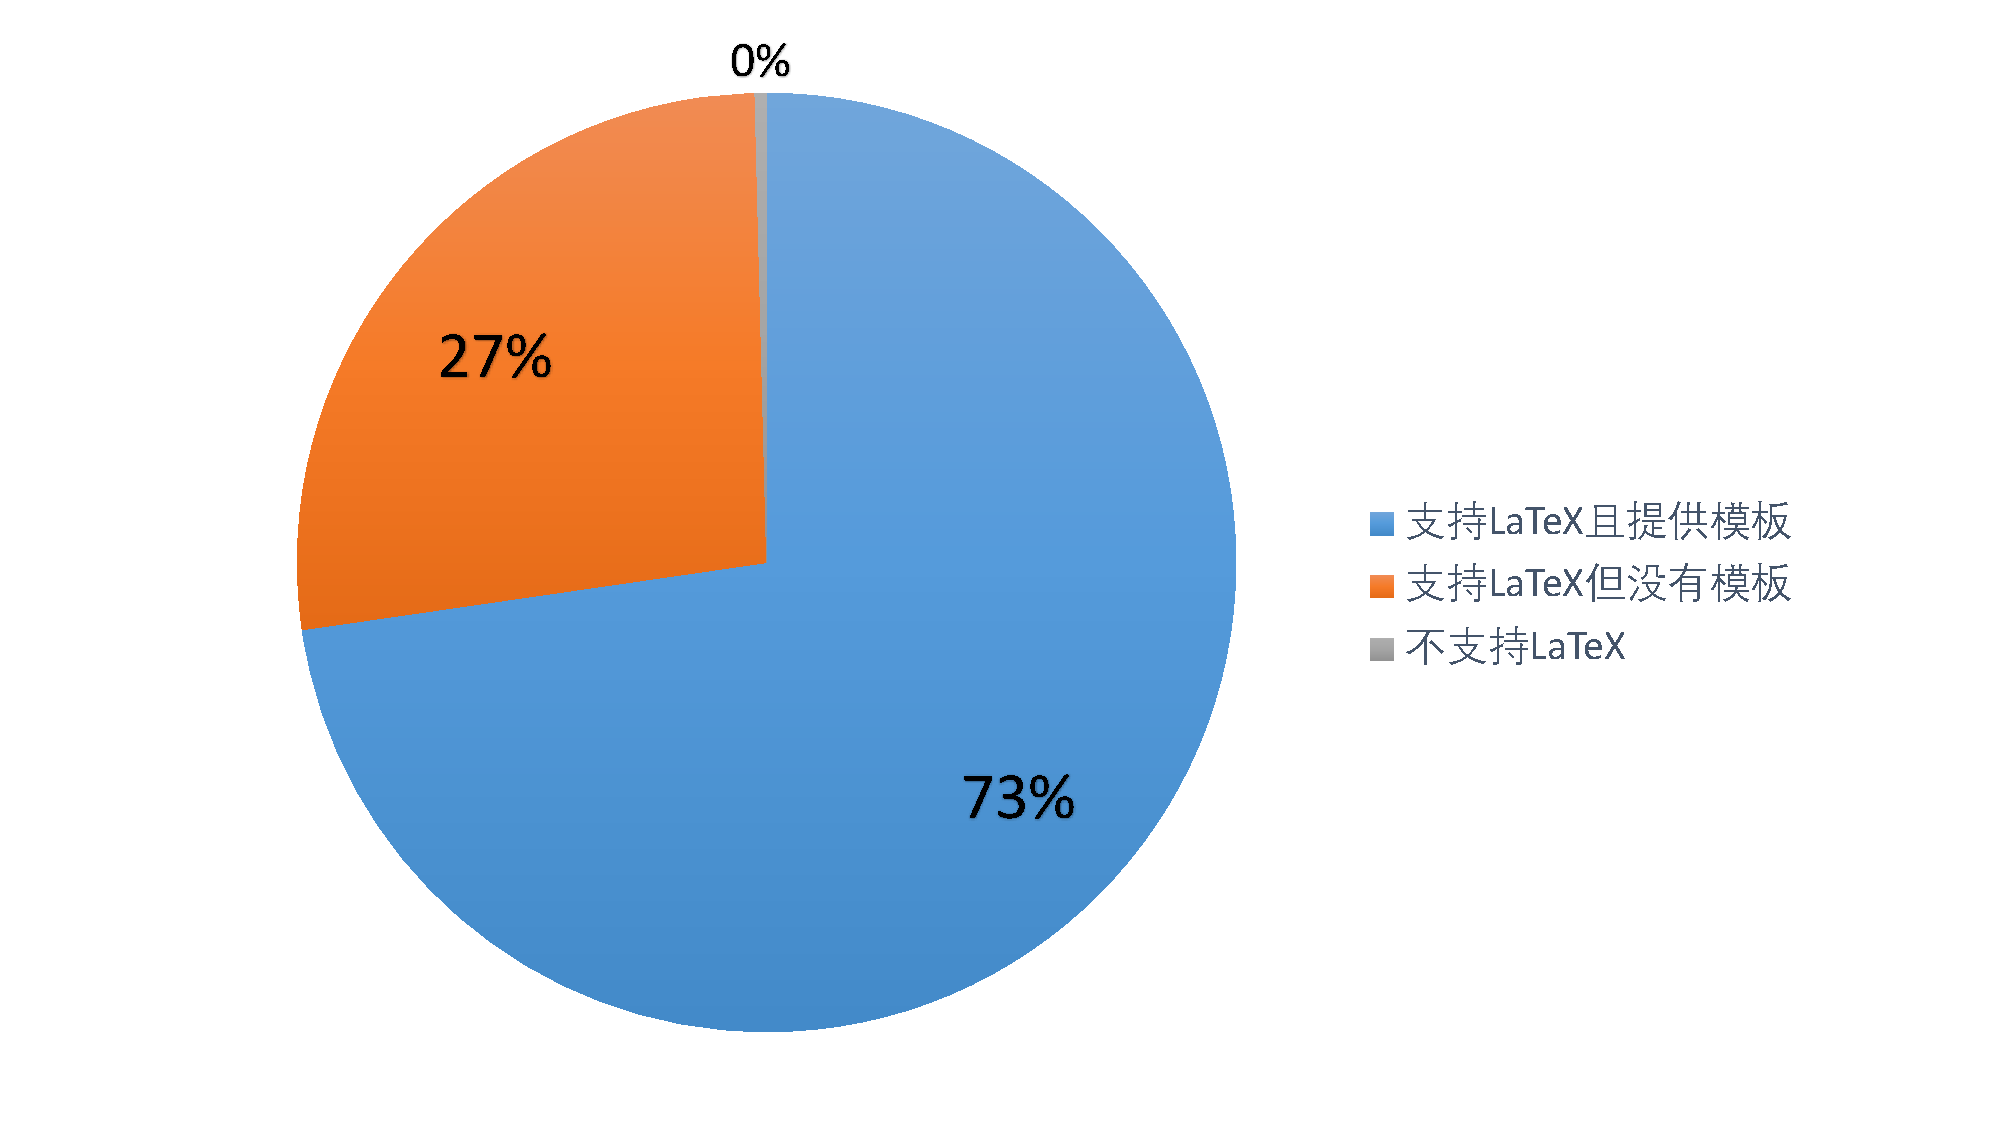
\includegraphics[width=\textwidth]{pubfig0}
\caption{顶级学术期刊出版社\TeX 支持情况}
\label{pubfig}
\end{figure}


调查显示样本库中所有顶级学术出版社均对使用\TeX 排版撰写的文章提供技术支持,其中73\%的学术出版社为作者提供\TeX 模板文件,极大便利了 \TeX 用户写作。(表\ref{pub}、图\ref{pubfig})
通过使用出版社提供的\TeX 模板文件,作者可以便利地排版出符合出版社格式要求和规范的论文,节约大量不必要的排版时间。

\ppt{\TeX:学术写作优势举例}
举个例子,在科研论文发表过程中,我们不可避免地会遇到学术文章需要由一部杂志改投其他杂志的情况,但是不同期刊的排版要求往往相差很大,从格式到文献引用方式可能都有不同,一点点修改调校则十分费时费力。好在,使用\TeX 来写作的论文可以直接改动文章排版时所依据的模板,这使得相同的文章在不同排版格式之间的便捷切换成为易事,这对提升研究人员投稿效率来说大有裨益。
\subsection{撰写毕业论文对\TeX 的需求}[Dissertation Typesetting with \TeX]\label{sec:texBene}
\ppt{\TeX 排版毕业论文:使用模板的益处}
在\ref{sec:whatistex}节中我们提到,\cquthesis 这一类定制的论文模板可以在很可观的程度上减轻\TeX 用户的排版负担——格式已经预置,标准已经订好,留给用户的事情便是组织内容以及将内容以符合\TeX 及\cquthesis 规范的方式编写出来,排版的任务则留给模板和\TeX 。

进一步地,对于各种用户需求,使用\TeX 对毕业论文进行排版还有以下好处:
\begin{itemize}
	\item 计算机系:代码着色和源程序引用,解决论文中插入的程序的版本之忧;
	\item 外语学院:多国语言文字支持,排版断句以自然段为单位\footnote{Word排版和断句以行为单位。},间距均衡,可读性高;
	\item 理工科:高效、美观、原生支持的数学公式、化学公式排版;
	\item 理工科:基于\texttt{.eps}和\texttt{.pdf}格式的矢量文件支持,矢量插图无限放大不失真;
	\item 更多美妙之处待你去体会和发掘。
\end{itemize}

总之,所有的用户都能花更少的时间排出更优秀的版面,而指导老师和学院也不用再烦心学生论文的格式问题,这便是使用\TeX 和论文模板排版毕业论文的突出优点。

\ppt{\TeX 排版毕业论文:国外高校情况}
在对具代表性五所世界名校(Oxford\cite{o1,o2}, Cambridge\cite{c1,c2}, Harvord\cite{h1,h2}, MIT\cite{m1}, Stanford\cite{s1,s2})的考察中,我们均在其官网上找到校方发布的毕业论文写作的\TeX 模版及\TeX 课程资源\footnote{可点击参考文献编号察看详情。}。值得注意的是,我们在由哈佛大学本科教务主任编写的《荣誉学士学位论文指南》\cite{h1}中找到了这样的内容“\LaTeX{} is recommended but not required.”(“我们推荐学生使用\LaTeX 撰写,不过,这并不是一个强制要求。”)

在以上所有学校中,校方都同时考虑了使用\TeX 及Word的同学的需求。

\ppt{\TeX 排版毕业论文:国内高校情况}
事实上,国内引进\TeX 已有数十年的历史,很多大学的大学生或研究生曾自发制作过自己学校的\TeX 模板。为了初步摸清国内大学\TeX 模板的开发和维护情况,笔者通过搜索引擎调研了国内主要大学(985高校及部分省份省会大学)的\TeX 模板开发情况、维护人员、项目地址、项目热度等信息。
截止2016年6月,国内主要大学(985高校及各省省会大学)的\TeX 模板情况如下\autoref{tab:domestic-statistics}所示:

\begin{longtable}[c]{cccccl}
	\caption{国内主要大学\TeX 模板维护情况统计}\label{tab:domestic-statistics}\\
	\toprule
	\ccell{学校}& \ccell{模板名称}& \ccell{维护人员}& \ccell{项目地址}& \ccell{热度} & \ccell{备注} \\
	\midrule\endfirsthead
	\multicolumn{6}{c}{续表~\thetable\hskip1em 国内主要大学\TeX 模板维护情况统计}\\
	\toprule
	\ccell{学校}& \ccell{模板名称}& \ccell{维护人员}& \ccell{项目地址}& \ccell{热度} & \ccell{备注}\\
	\midrule
	\endhead
	\hline
	\multicolumn{6}{r}{续下页}
	\endfoot
	\endlastfoot
	中国科学院研究生院 & CASthesis & 吴凌云 & \href{http://www.ctex.org/PackageCASthesis}{CTeX页面}\footnote{点击可访问,下同。} & 5 & {\zihao{-5}历史悠久,始祖模板之一} \\
	清华大学 & thuthesis & Ruini Xue & \href{https://ctan.org/pkg/thuthesis}{CTAN页面} & 5 & {\zihao{-5}维护良好,始祖模板之一,用户基数大} \\
	上海交通大学 & SJTUThesis & weijianwen & \href{https://github.com/weijianwen/SJTUThesis}{Github页面} & 5 & {\zihao{-5}维护良好,用户基数大} \\
	南开大学 & NKT & 孙文昌 & \href{http://202.113.29.3/~sunwch/tex/tex.htm}{学校网站} & 4 & {\zihao{-5}数学系教授维护} \\
	电子科技大学 & uestcthesis & Shi Fu­jun& \href{https://www.ctan.org/pkg/uestcthesis}{CTAN页面} & 4 & {\zihao{-5}关注度很不错,研究生院认证,维护略欠缺\footnote{\href{https://www.ctan.org/pkg/uestcthesis}{CTAN版本}最后维护于2013年5月底,好在\href{https://github.com/shifujun/UESTCthesis}{Github版本}维护活跃。学校有\TeX 社区。}} \\
	北京航空航天大学 & BUAAthesis & BHOSC & \href{https://github.com/BHOSC/BUAAthesis}{Github页面} & 4 & {\zihao{-5}} \\
	南京大学 & nju-thesis & Haixing-Hu & \href{https://github.com/Haixing-Hu/nju-thesis}{Github页面} & 4 & {\zihao{-5}历史悠久,最早追溯到6年前,分支众多\footnote{4个分支,现在最热的分支维护得不错,没上CTAN有点可惜。}} \\
	中国科学技术大学 & USTCThesis & ustctug & \href{https://github.com/ustctug/ustcthesis}{Github页面} & 4 & {\zihao{-5}模板代码和运营都很棒\footnote{ustctug是一个很有实力的社团。}} \\
	北京大学 & pkuthss & Casper Ti. Vector & \href{http://ctan.org/pkg/pkuthss}{CTAN页面} & 3 & {\zihao{-5}} \\
	北京师范大学 & BnuThesis & henrysting@gmail.com & \href{http://gerry.lamost.org/blog/?p=811}{个人博客} & 3 & {\zihao{-5}清华系} \\
	山东大学 & sduthesis & Liam Huang & \href{http://www.ctan.org/pkg/sduthesis}{CTAN页面} & 3 & {\zihao{-5}清华系,起步相对早,本硕博支持不全} \\
	湖南大学 & HNUThesis & 杜家宜 & \href{http://www.hnubbs.com/forum.php?mod=viewthread&tid=790603}{学校论坛} & 3 & {\zihao{-5}清华系,不支持本科} \\
	华中科技大学 & hustthesis & hust-latex & \href{https://github.com/hust-latex/hustthesis}{Github页面} & 3 & {\zihao{-5}学校建有CTAN镜像,模板有些瑕疵\footnote{正在谋划提交CTAN.}} \\
	哈尔滨工业大学 & PlutoThesis & dustincys & \href{https://github.com/PlutoThesis}{Github页面} & 3 & {\zihao{-5}历史悠久,分硕博版本和本科版本} \\
	国立台湾大学 & ntu-thesis & tzhuan & \href{https://github.com/tzhuan/ntu-thesis}{Github页面} & 3 & {\zihao{-5}维护良好,用xeCJK解决方案} \\
	武汉大学 & WHUBachelor & 黄正华 & \href{http://aff.whu.edu.cn/huangzh/}{学校网站} & 2 & {\zihao{-5}作者为武大老师,LaTeX经验丰富\footnote{课件使用Beamer来做,模板完成度不高,仅支持本科生。}} \\
	中国海洋大学 & ZwPhdThesis & 周炜 & \href{http://blog.sciencenet.cn/blog-453771-456252.html}{个人博客} & 2 & {\zihao{-5}完成度较低,仅支持博士论文} \\
	西北工业大学 & nwputhesis & Wang Tianshu & \href{http://code.google.com/p/nwputhesis/}{Google Code} & 2 & {\zihao{-5}维护停滞,但是有热度} \\
	东南大学 & SEUThesis & 许元 & \href{http://www.ctan.org/pkg/seuthesis}{CTAN页面} & 2 & {\zihao{-5}本身质量不错,但是没有宣传好和维护好} \\
	华南理工大学 & scutthesis & Alwin Tsui & \href{https://github.com/alwintsui/scutthesis}{Github页面} & 2 & {\zihao{-5}面向Lyx写的一个模板,这点很有意思} \\
	四川大学 & scu\_thesis\_template & cuiao & \href{https://github.com/dahakawang/scu_thesis_template}{Github页面} & 2 & {\zihao{-5}质量一般\footnote{另外有一个,点击访问\href{https://github.com/cuiao/SCU_ThesisDissertation_LaTeXTemplate}{Github页面}}} \\
	中国国防科学技术大学 & nudtpaper & Liu Benyuan & \href{https://github.com/liubenyuan/nudtpaper}{Github页面} & 2 & {\zihao{-5}代码历史悠久,现在的版本是传承下来的} \\
	复旦大学 & FDU-Thesis-Latex & Pandoxie & \href{https://github.com/Pandoxie/FDU-Thesis-Latex}{Github页面} & 2 & {\zihao{-5}上次维护为2年前,硕博双版本} \\
	天津大学 & TJUThesis  & 张井、余蓝涛 & \href{https://github.com/xnth97/TJUThesisLatexTemplate}{Github页面} & 2 & {\zihao{-5}教务处发文介绍推荐} \\
	浙江大学 & write\_with\_LaTeX & Monster, Hamburger & \href{https://github.com/ZJU-Awesome/write_with_LaTeX}{Github页面} & 2 & {\zihao{-5}起步很早,版本很多,代码相对老一些\fancyfoot{,部分分支为清华系。}} \\
	同济大学 & TongjiThesis & gareth@tongji.net & \href{https://sourceforge.net/projects/tongjithesis/}{Sourceforge} & 2 & {\zihao{-5}清华系,最后维护:2009年} \\
	西安交通大学 & XJTUthesis & multiple1902 & \href{https://code.google.com/archive/p/xjtuthesis/}{Google Code} & 1 & {\zihao{-5}起步早,有三个平行项目\footnote{由于学校的支持欠缺,基本上都停止了。这是\href{https://code.google.com/archive/p/xjtuthesis/wikis/Letters.wiki}{一个明显的项目因为缺乏学校支持而失去活力的例子}。}} \\
	中山大学 & sysu\_thesis & 陈颂光 & \href{https://github.com/chungkwong/sysu_thesis}{Github页面} & 1 & {\zihao{-5}代码完成度不错,仅支持本科} \\
	兰州大学 & LZUthesis & mosesnow & \href{https://github.com/mosesnow/LZUthesis}{Github页面} & 1 & {\zihao{-5}中科院系,另外支持Lyx} \\
	东北大学 & NEU\_PHD\_Template & 艾均 & \href{https://github.com/NobodyLiveForever/NEU_PHD_Template}{Github页面} & 1 & {\zihao{-5}上次维护为3年前,仅支持博士} \\
	大连理工大学 & DLUT & whufanwei, yuri\_1985 & \href{https://github.com/whufanwei/}{Github页面} & 1 & {\zihao{-5}上次维护为4年前,分硕博双版本} \\
	厦门大学 & xmu-template & 王玮玮 & \href{https://github.com/wwwxmu/-Latex-}{Github页面} & 1 & {\zihao{-5}模板的代码很简陋\footnote{只涉及了封面和摘要,章节、目录等都没有涉及。厦门大学开有\LaTeX 选修课程。}} \\
	中国人民大学 & ructhesis & ZebinWang & \href{https://github.com/ZebinWang/ructhesis}{Github页面} & 1 & {\zihao{-5}} \\
	华东师范大学 & ecnuthesis & 邓沛 & \href{https://sourceforge.net/projects/ecnuthesis/}{Sourceforge} & 1 & {\zihao{-5}代码思路不错,最后维护:2012年} \\
	重庆大学 & CQUThesis & 李振楠 & \href{https://www.ctan.org/pkg/cquthesis}{CTAN页面} & 1 & {\zihao{-5}刚刚开启,还需要生态建设\footnote{其实,在2014年左右,我校学子陈关才开发过名为CQU的毕业论文模板,托管于\href{https://code.google.com/archive/p/cqu/}{Google Code},不过这个项目已经很久没有维护了。}} \\
	吉林大学 & jluthesis & Zhang Yinhe & \href{https://code.google.com/archive/p/jluthesis/}{Google Code} & 0 & {\zihao{-5}最后维护:2009年} \\
	云南大学 & ynuthesislyx & cherrot & \href{https://github.com/cherrot/ynuthesislyx}{Github页面} & 0 & {\zihao{-5}清华系,基于Lyx,仅本科\footnote{最后维护于3年前。}} \\
	北京理工大学 &  &  &  & 0 & {\zihao{-5}建有CTAN镜像} \\
	中国农业大学 &  &  &  & 0 & {\zihao{-5}有人尝试过} \\
	中央民族大学 &  &  &  & 0 & {\zihao{-5}} \\
	中南大学 &  &  &  & 0 & {\zihao{-5}有人尝试过,但是不成系统} \\
	西北农林科技大学 &  &  &  & 0 & {\zihao{-5}} \\
	广西大学 &  &  &  & 0 & {\zihao{-5}} \\
	香港大学 &  &  &  & 0 & {\zihao{-5}} \\
	澳门大学 &  &  &  & 0 & {\zihao{-5}} \\
	西藏大学 &  &  &  & 0 & {\zihao{-5}} \\
	\bottomrule
\end{longtable}

在解读数据时,以下几点也许需要注意:
\begin{itemize}
	\item “热度”一项由笔者综合评判而得,0为无热度,即认为几乎不会有人使用、讨论、修订、维护相关模板,1$ \sim $5为有热度,数值越大,热度越高,其中规定以清华大学模板\textsc{THUThesis}的热度为5。热度的判定基于以下因素:模板最近维护时间和历史维护频率、关于模板的相关讨论(例如Github Issues)、模板代码质量、模板功能完全程度、模板是否被其他模板所模仿和引用\footnote{清华大学的模板\textsc{THUThesis}、上海交通大学的模板以及哈尔滨工业大学的模板便是有力的例子,很多学校的模板都是在它们的基础上再开发而来。这当中也体现了开源软件的优越性质。}、模板是否模仿和引用其他模板\footnote{例如\cquthesis 即为清华系模板。}、学校支持程度、\TeX 社群维护质量、学校是否维护有CTAN镜像等;
	\item 从模板的托管位置也能看出一些特点,例如:1. 至今仍然托管于Google Code的模板一般都是开发得很早(先驱者),但已经停止维护很久的模板\footnote{Google Code于2015年8月底进入只读模式,如果项目仍然有维护,一般会被迁移到Github。};2. 很多的模板托管于Github,看得出大部分开发者都有此共识:论文模板这一类产品需要和用户保持交流(需求变化、学校规定更新等);3. 托管于CTAN的模板一般都有着不错的质量\footnote{模板上传到CTAN就意味着模板有使用手册,而有使用手册的模板的维护力量一般都不会太差。};4. 有的模板托管于学校相关网站,这一般都会给模板带来不错的关注度。
\end{itemize}


\ppt{\TeX 排版毕业论文:学校支持和认可的必要性}
从以上数据中,我们可以得出一些初步结论:
\begin{enumerate}
	\item \TeX 作为舶来品,其传播和使用与学校当中的科研人员的使用需求相关度高,科研能力强,投稿需求大的学校(在\ref{sec:jounaldemands}节中我们讨论过期刊投稿中使用\TeX 作为文章接受格式的比例和成因),对\TeX 的认知更加全面,从而在学生当中更可能会有愿意和能够进行模板开发的先行者;
	\item 很多历史悠久的模板都没能撑下来,这和学校\TeX 用户稀少,社群凝聚力差,模板维护者放弃维护息息相关;
	\item 几乎没有学校会以官方的身份去开发模板,但是学校可以对模板进行测试、认证以及推荐;
	\item 学校的支持和认可是十分必要的,学校的支持会带来源源不断的\TeX 用户,这使得每年毕业季模板都会有人使用,从而获得持续的反馈;学校的认可则会稳定\TeX 用户们的心,让他们确信,在花功夫习得\TeX 的使用方法后,他们会有用武之地\footnote{西安交通大学的模板开发是\href{https://code.google.com/archive/p/xjtuthesis/wikis/Letters.wiki}{一个明显的项目因为缺乏学校支持而失去活力的遗憾}。}。同时,这也是对模板作者的鼓励和推动。
\end{enumerate}


\subsection{\TeX 的其他典型运用环境}[Other Typical Application of \TeX]

\ppt{数模竞赛:TeX}
数模竞赛可以说是对国内\TeX 运用作用范围最广的催化剂了,很多同学都因此认识并学习了\TeX 。无论是\href{https://github.com/latexstudio/CUMCMThesis}{全国大学生数学建模竞赛(CUMCM)}或是\href{http://www.latexstudio.net/archives/25}{美国大学生数学建模竞赛(ACM)}都有由国内\TeX 爱好者制作的出色模板\footnote{实际上有很多爱好者制作了很多版本,链接中给出了典型。}。

%****第三章:接受TeX毕业论文*****
\section{接受使用\TeX 撰写的毕业论文}[Advices on Acceptance for Dissertation Typesetting with \TeX]
\subsection{提议原因}[Reasoning]
\ppt{引入\TeX :开明之举}
在第\ref{sec:texBene}节中,我们讨论了在学术论文排版时使用\TeX 的优越性。\cquthesis 使得毕业生能够以很低的排版时间代价得到格式规范,排版质量高,索引目录齐全,美观大方的毕业论文。但是,\TeX 对于许多同学来说却是百分百的新事物(尽管\TeX 发行于1978年),学校官方的表态无疑会为许多对\TeX 有兴趣却烦恼没有用武之地的同学提供学习的动力。

\ppt{引入\TeX :民心所向}
当前,我校教务处以及研究生院对是否接受\TeX 撰写的毕业论文这一问题态度模糊。在我校民主湖论坛上,针对这一问题有很多讨论,以下是一些典型的帖子:
\begin{itemize}
	\item \href{http://www.cqumzh.cn/bbs/forum.php?mod=viewthread&tid=830829}{请投票支持论文采用\LaTeX 排版}
	\item \href{http://www.cqumzh.cn/bbs/forum.php?mod=viewthread&tid=830608}{[讨论] 重大的博士论文为什么木有\LaTeX 模版?}
	\item \href{http://www.cqumzh.cn/bbs/forum.php?mod=viewthread&tid=264031}{[理工科学] 有用\LaTeX 写论文的吗?交流一下 }
	\item \href{http://www.cqumzh.cn/bbs/forum.php?mod=viewthread&tid=931065}{博士毕业论文用\LaTeX 排版,之后的提交什么的会麻烦么?}
	\item \href{http://www.cqumzh.cn/bbs/forum.php?mod=viewthread&tid=936958}{重庆大学自己的毕业论文\LaTeX 模板来啦!}
	\item \href{http://www.cqumzh.cn/bbs/forum.php?mod=viewthread&tid=615852}{[编程] [求助]关于\LaTeX}
	\item \href{http://www.cqumzh.cn/bbs/forum.php?mod=viewthread&tid=818609}{被\LaTeX 所征服}
\end{itemize}

帖子的时间跨度从2006年至今,可以看出,至少在十年以来,我校师生中一直存在着\TeX 用户。在帖子中,他们的情感主要着力于以下几点:1. 认识到\TeX 很强大,主观上很想使用\TeX 进行毕业论文排版;2. 对教务处(本科生)或研究生院(研究生)是否接受使用\TeX 排版的论文心存顾虑,感到烦恼;3. (研究生)对研究生院毕业论文收费排版的现状\footnote{笔者对研究生院要求绝大多数研究生以1元/页的价格购买官方指定的排版服务的做法深表遗憾。}感到愤怒和无奈;4. 学习\TeX 遇到困难,感到求助无门。

在帖子\href{http://www.cqumzh.cn/bbs/forum.php?mod=viewthread&tid=830829}{请投票支持论文采用\LaTeX 排版}中,发帖人luoluo114\footnote{按照民主湖论坛的账号政策,民主湖论坛内的用户都是重庆大学学子。}发起了投票,他说道\footnote{原文引用,不改变错别字或错误用法,例如“latex”应该写为“LaTeX”,或者“\LaTeX ”,下同。}:

\begin{quotation}
	为避免我们的下一届学弟学妹身受格式痛苦,我觉得有必要发起该投票。latex其优点是有目共睹的,希望研院发起这样一个模板,或者承认latex格式的论文,让大家把精力应用于论文质量而不是格式本身。
	
	本人曾用word写毕业论文,因参考文献标号不是从1开始而花在修改编号上的时间用了一天。 而利用latex,仅仅是几分钟的事情。
\end{quotation}

在参与投票的246名重大学子中,有162名投票希望使用\LaTeX 排版,51名希望使用Word排版,33名没有表态,票数之间大小关系如\autoref{fig:tex-word-vote}所示。

\begin{figure}[tbh]
\centering
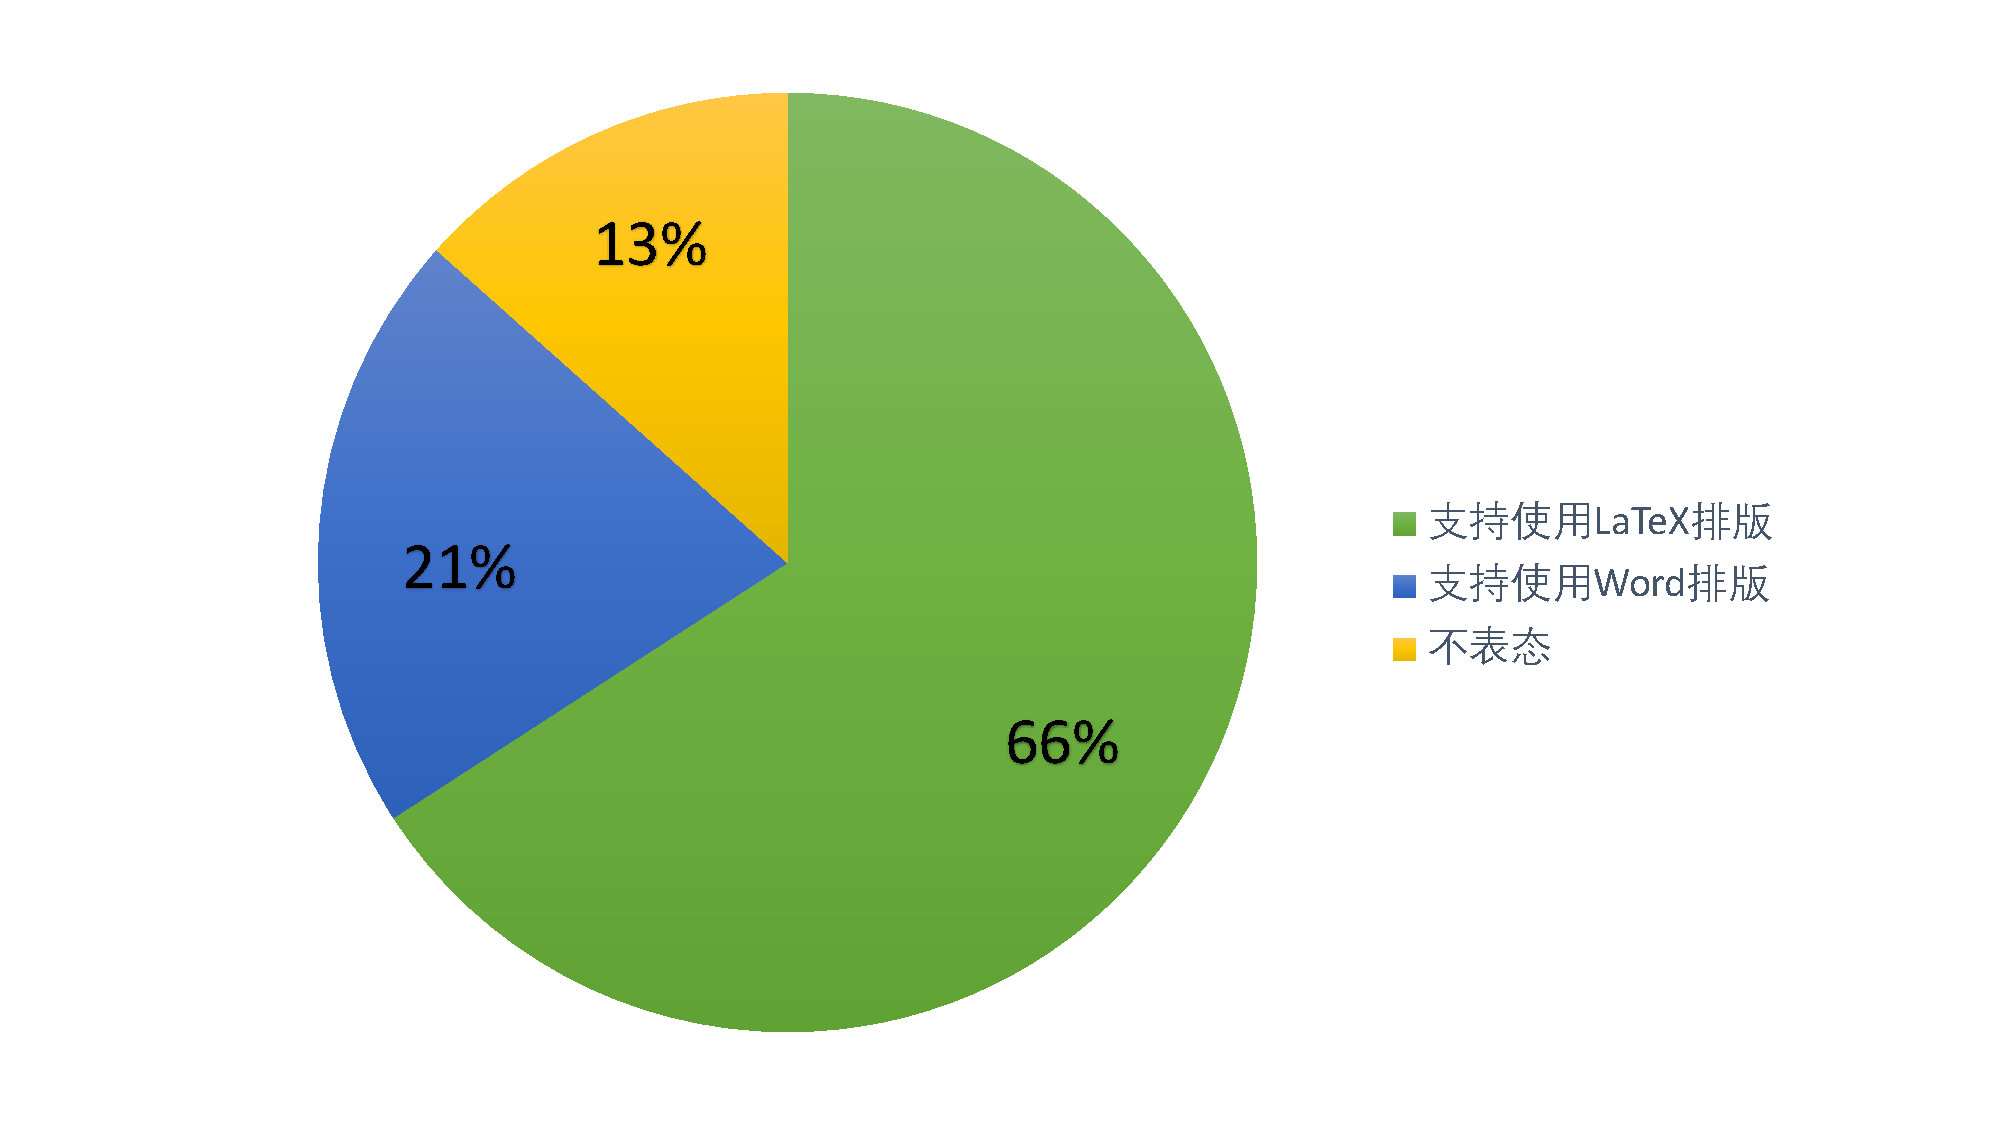
\includegraphics[width=\linewidth]{figures/TeX-Word-Vote}
\caption{民主湖中使用\LaTeX 进行毕业论文排版的支持率}
\label{fig:tex-word-vote}
\end{figure}

笔者另外节录了一些有思想性的观点,以飨读者:
\begin{quotation}
	这个建议官方做不是太靠谱,一般学校都是latex版面的爱好者自己做的 。
	很多学校都有自己的版本,上海交大,中国科大等,都是基于CASthesis 的。
	其实论文格式要求都差不多,拿过来修改下就可以了。
	用latex写论文,还是比较方便的,不太熟悉 tex的人照模块做基本都能做到。
	\par\hfill ——paulsum
	
	latex入手较慢,不过常用的功能很好掌握。
	熟练以后论文排版很快,而且整齐划一。
	\par\hfill ——cqustone
	
	Latex最重要的是排版规范,格式基本不会出错,如果学校能组织一帮同学做个模板,或者说承认同学的Latex排板,会给写论文带来极大方便。因为你关注是论文本身,而不会再去关注格式!这一点word是做不到的。
	
	word编号是没有问题,但我想大部分同学都遇到过文章长了之后格式不对的情况,什么编号缩进不对,前后文字体不对等等。而对于latex来说,你只需要知道此处应该有编号就可以了,缩进字体这些提供的模板自然会帮你处理。
	\par\hfill ——chengfzy
	
	这不是砸人家饭碗吗?你知道采用LATEX编辑,(研究生院指定的排版机构)要少挣多少钱不?
	\par\hfill ——sxkcqu
	
	最近在用这个软件写论文,感觉功能强大,但是又比较难学,经常为一个小问题卡壳,希望有同样爱好者交流一下!
	\par\hfill ——woodhead
	
	有没有什么地方必须提交word版的?用Latex排版然后提交生成的pdf可以么?有毕业了的师兄师姐是用的网上那个重大的Latex模板完成毕业论文的么?
	\par\hfill ——dashashi
	
	重大不让。如果可以的话省去很多麻烦。公式这些都不用去敲了。也不用去为格式操心,latex格式是固定的,不会出错。
	\par\hfill ——240536501
	
	前段时间了解了一些基础知识,现在意识到它的强大了。不在于能记忆多少,只要能很好的利用template完成自己的工作,那么Latex就为你节约了时间。这是它设计的目的之一。
	
	期待重大学位论文退出Latex的模板。
	\par\hfill ——八五折
	
	为设计者nanmu点赞!
	
	同时也希望研究生院相关部门大力支持,并推进其完善以至于形成正式版本,让更多的同学受益。
	
	Latex的广泛性和重要性不言而喻(基本覆盖了所有知名的国际期刊和出版集团,国内期刊也在大力推广),既然有专业人士用于尝试(如计者nanmu),相关部门更该顺势推进,成功推广必然对研究生学位论文相关工作起到巨大促进作用。而如果对此不予支持,甚至提出质疑,着实让人遗憾!
	
	试想这样一个场景,一位在国际知名期刊发表多篇高级别论文的博士生(小论文均为Latex版本),却要在答辩之前,花费大量时间精力用于研究latex与word之间的转化问题(笔者有过此经历,可谓“深受其害”),实在让人抓狂。希望这种情况不要再发生在各位在读的小伙伴身上了!
	\par\hfill ——supermtd
\end{quotation}

综合上述内容,学校联合教务处、研究生院表态接受使用\TeX 撰写的毕业论文是民心所向,也是引入先进工具先进思想的开明之举。

\subsection{依赖条件}[Dependencies]
\begin{enumerate}
	\item 论文存档方面,PDF文件本身的设计意图之一便是用于存档\cite{pdfISO},其格式稳定、规范\footnote{ISO 19005-3:2012},高度向后兼容,适合文件长期存档;
	\item 论文查重方面,大部分论文查重机构都能够对PDF文件格式的论文进行查重工作;
	\item 学校开设\TeX 培训课程(参阅第\ref{sec:texCourses}章);
	\item 学校完成CTAN镜像搭建(参阅第\ref{sec:ctanMirror}章)。
\end{enumerate}

\subsection{具体措施}[Detailed Measures]
措施可分为三步,表态、测试和推荐、维护。

\begin{enumerate}
	\item 表态:学校联合教务处、研究生院发文,表示接受使用\TeX 排版的PDF格式的论文,并确认提交PDF格式的论文和提交Word格式的论文完全等效,同时规定,无论论文的文件格式是什么,排版方式是什么,其格式以及书写规范都要符合重庆大学《重庆大学本科设计(论文)撰写规范化要求(2007年修订版)》和《重庆大学博士、硕士论文撰写格式标准(2007年修订版)》的要求;
	\item 测试和推荐:学校组织格式审查委员会对\cquthesis 的排版情况进行审查,确认其排版合规的情况下,在教务处和研究生院的毕业论文系统中添加\cquthesis 的说明介绍、用户文档和下载地址,起到对\TeX 用户的指导效果;
	\item 维护:学校保持对CTAN镜像的维护(参阅第\ref{sec:ctanMirror}章),并且保持对\TeX 培训课程(请参阅第\ref{sec:texCourses}章)的支持,如此这般,重庆大学师生的学术写作水平会在一定程度上得到长足提升,并且生生不息。
\end{enumerate}

\cquthesis 的技术维护由\href{https://github.com/nanmu42/}{李振楠}和\href{http://jq.qq.com/?_wv=1027&k=2HvYu95}{重庆大学\TeX 用户组}进行。
%****第四章:开设TeX课程*****
\section{开设\TeX 选修课程}[Advices on Offering \TeX Courses and Resources ]\label{sec:texCourses}
\subsection{提议原因}[Reasoning]

目前,我校的“计算机基础”必修课向全体学生提供了 Office Word 软件操作方法的全面训练,而学校IT中心也出资为全体师生取得了Office Word的集体正版授权,为师生提供了极大便利,这些举措在全国高校中堪称领先。

在前文中,我们陈述了\TeX 在学术写作和出版中的重要性和高效性。将高质量的、高效的资源充分暴露给学习者,使其能够自由选择适合自己的学习与实践方式,才能发挥其积极的挖掘精神,最大化学习与实践效果。因此,我校有必要也有需要面向本科生(毕业论文撰写需求)和研究生(期刊投稿需求)推出\TeX 相关课程培训,这会提高我校师生在学术写作领域的素养,同时对学生创新意识与编程思维的开发培养有利。

再者,学校开设\TeX 相关课程能够大大降低初学者入门难度,降低其学习成本,这对学生掌握知识和撰写论文皆有裨益。

\subsection{依赖条件}[Dependencies]
\begin{enumerate}
	\item 基础建设方面,我校需要拥有自己的CTAN镜像,以便利我校师生获取\TeX 软件和使用文档等相关资源;
	\item 师资方面,我校计算机系和数学系当中应该有一部分教授、讲师为经验丰富的\TeX 用户;
	\item 学校政策方面,接受\TeX 撰写的毕业论文(本科生、研究生、博士生)会增进学生学习\TeX 的动力;
	\item 课程研发方面,可依托重庆大学大学生创新实践中心和重庆大学研究生创新实践基地为实验田(他们也是论文投稿的主力军),逐渐向全校推广。
\end{enumerate}

\subsection{具体措施}[Detailed Measures]
\ppt{硬件建设}
措施可分为硬件建设和软件建设,硬件建设方面:
\begin{itemize}
	\item 完成CTAN镜像搭建(参阅第\ref{sec:ctanMirror}章);
	\item 在向本科生、研究生授课的计算机机房中预装\href{https://en.wikipedia.org/wiki/TeX_Live}{\TeX Live}发行版、\href{http://www.texstudio.org/}{TeX Studio}编辑环境;
\end{itemize}

\ppt{软件建设}
软件建设方面:
\begin{enumerate}
	\item 在校内征集有经验的、对\TeX 有热情的老师;
	\item 为老师提供研讨环境和资源,以方便其制定教案和教材\footnote{可以参考以下资源:
		\href{http://bbs.ctex.org/forum.php?mod=viewthread&tid=68619}{《\LaTeX 排版学习笔记》}、
		\href{http://texdoc.net/texmf-dist/doc/latex/lshort-chinese/lshort-zh-cn.pdf}{《一份不太简短的\LaTeXe 介绍》}、
		\href{http://ptgmedia.pearsoncmg.com/images/9780201362992/samplepages/0201362996.pdf}{《The \LaTeX Companion》}(此处为样张,可在\href{https://www.amazon.com/dp/0201362996}{亚马逊美国}购买)、
		\href{https://www.amazon.cn/dp/B00D1APK0G}{《\LaTeX 入门》}、
		\href{https://www.amazon.cn/dp/B019ERSEAW/}{《21世纪高等院校通识教育规划教材:\LaTeX 科技论文写作简明教程》}。};
	\item 以重庆大学大学生创新实践中心和重庆大学研究生创新实践基地作为试验田进行授课和反馈,可考虑将课程内容与“学术写作”课程联动或合并;
	\item 在教案和教材成熟后,面向全校本科生开设选修课(对毕业论文撰写有利),面向全校理工科研究生开设必修课(对期刊投稿及毕业论文撰写有利)。
\end{enumerate}

需要注意的是,课程应当安排足够的上机课时以及实践型作业。
%****第五章:建立CTAN镜像*****
\section{建立重庆大学CTAN镜像}[Advices on Setting Up a CTAN Mirror]\label{sec:ctanMirror}
\subsection{提议原因}[Reasoning]
\ppt{基础建设}
让用户轻松便捷地下载到\TeX 软件及相关内容是壮大我校\TeX 用户群体的第一步,它的角色如同基础建设一般。

\ppt{CTAN}
作为自由软件,\TeX 的维护工作由全世界的\TeX 爱好者们合力完成,软件分发由CTAN主导完成。CTAN是\href{https://www.ctan.org/}{Comprehensive \TeX Archive Network}的简称,它向全球用户提供\TeX 发行版、宏包、模板、使用文档、源代码、应用程序等文件的下载。

CTAN并不是“一个”网站,它由一个核心站点\footnote{\url{http://dante.ctan.org},由德国\TeX 用户组赞助,Rainer Schoepf主导维护。}和许许多多镜像站点\footnote{站点列表详见\url{https://www.ctan.org/mirrors}。}构成。镜像站点定期与核心站点同步,与核心站点一同向公众提供\TeX 相关资源的下载。使用镜像站点有两个显而易见的优势:

\begin{itemize}
	\item 对于分散在全球各地的用户来说,用户可以选择距离自己最近、网络连通性最好的镜像,从而实现高速下载;
	\item 对于CTAN自身而言,镜像可以为核心站点和其他镜像分担流量,降低整个CTAN网络的压力。
\end{itemize}

\ppt{CTAN:中国}
目前,在中国有4个官方镜像,它们分别是\href{http://mirrors.tuna.tsinghua.edu.cn/CTAN/}{清华大学}、\href{http://mirrors.ustc.edu.cn/CTAN/}{中国科学技术大学}、\href{http://mirrors.hust.edu.cn/CTAN/}{武汉理工大学}、\href{http://mirror.lzu.edu.cn/CTAN/}{兰州大学}。它们的存在使得中国教育网用户和公众网用户享受到了高速便利的\TeX 内容下载。值得注意的是,上述镜像分布于中国北部、中部及西北地区,西南地区还没有镜像。

\ppt{CTAN:重庆大学}
综上所述,倘若我校适配相关资源(我校已有硬件设施,不需要追加投入,仅需要进行技术和软件方面的调整),进行CTAN的镜像工作,对我校师生乃至中国西南的\TeX 用户来说都是重大利好。

\subsection{依赖条件}[Dependencies]
\ppt{蓝盟}
硬件和技术方面,我校\href{http://lanunion.cqu.edu.cn/}{蓝盟}已经在维护运营重庆大学开源镜像站\footnote{\url{https://mirrors.cqu.edu.cn/}},该站点收录了 CentOS、Archlinux、CentOS、Ubuntu等多个发行版的镜像,另有CPAN等与CTAN结构相似的开源镜像。可以说,我校具备相关硬件和技术条件。

外部支持方面,CTAN一直都欢迎新镜像的加入,在完成相关技术工作后,CTAN会将我校镜像站点加入其官方镜像列表。

\subsection{具体措施}[Detailed Measures]
CTAN提供了\href{https://www.ctan.org/mirrors/register/}{一份详细的操作方案}\footnote{\url{https://www.ctan.org/mirrors/register/}},简略而言,方案包含下列四个步骤:
\begin{enumerate}
	\item 在服务器上提供Web和/或FTP服务;
	\item 使用rsync命令从核心站点拉取数据;
	\item 将rsync命令作为cron job每日执行,保持我校镜像与核心站点同步;
	\item 注册成为官方镜像,加入官方镜像列表。
\end{enumerate}

视我校实际情况,蓝盟方面会按现有条件进行具体操作,望学校给予接洽和支持为宜。蓝盟的兄弟(姐妹),如果你正读到这里,请接受我们的致意和感谢,谢谢你们!
%****第六章:结语*****
\section{结语}[Conclusion]

本提案从介绍排版系统\TeX 的背景和特点开始,从研究生期刊论文投稿以及毕业生毕业论文排版工作这两个维度阐述了引入\TeX 作为一种与Office Word平行的写作系统的优势和必要性,最终提出一套基于我校实际情况、有效可行的实施方案:接受使用\TeX 撰写的毕业论文、开始\TeX 选修课程以及建立重庆大学CTAN镜像。

将\TeX 这个美好的、强大的写作排版工具充分推荐给重大师生,对我们的学术写作水平提高大有裨益,既有利于研究生、博士生的论文投稿工作,又有利于重大全体学子的毕业论文排版工作。长远来看,这对挖掘学生的的创新潜质,调动创新意识,营造创新氛围,培养一批拥有全球视野、掌握核心竞争力的拔尖创新人才极有帮助。

“必人才日出,然后事业日新;必事业日新,然后生机永畅。”

愿母校在“双一流大学”建设计划中走出高度,走出水平。
%=======附件部分========
% 参考文献
\clearpage
\bibliographystyle{cqunumerical}
\bibliography{ref/bluescas,ref/nanmu}
% 关键词索引
\printindex
\end{document}